\chapter{Design and Implementation}
Two separate facets of Djangorifa have been developed:
\begin{itemize}
\item Reports Management
\item Facilities Management
\end{itemize}

This chapter will provide an overview of how the components fit together, and detail the shared components of the system.

\section{Overview}
\label{sec:di:ov}

Figure~\ref{fig:di:uml} is the UML Diagram of the overview of the system. There are other apps which have not been shown because they are not required for understanding how the system fits together. They are, however, discussed later. Note that this was created with the command:

\begin{figure}[thp]
	\centering
	\begin{tabular}{c}
	\begin{lstlisting}[label={lst:graph_models},breaklines=true]
	./manage.py graph_models -n -d -g -e -o overview.png reports facilities auth registration users reports taarifa_config sites
	\end{lstlisting}
	\end{tabular}
	\caption{Code to generate overview UML}
\end{figure}

\begin{figure}[h]
\centering
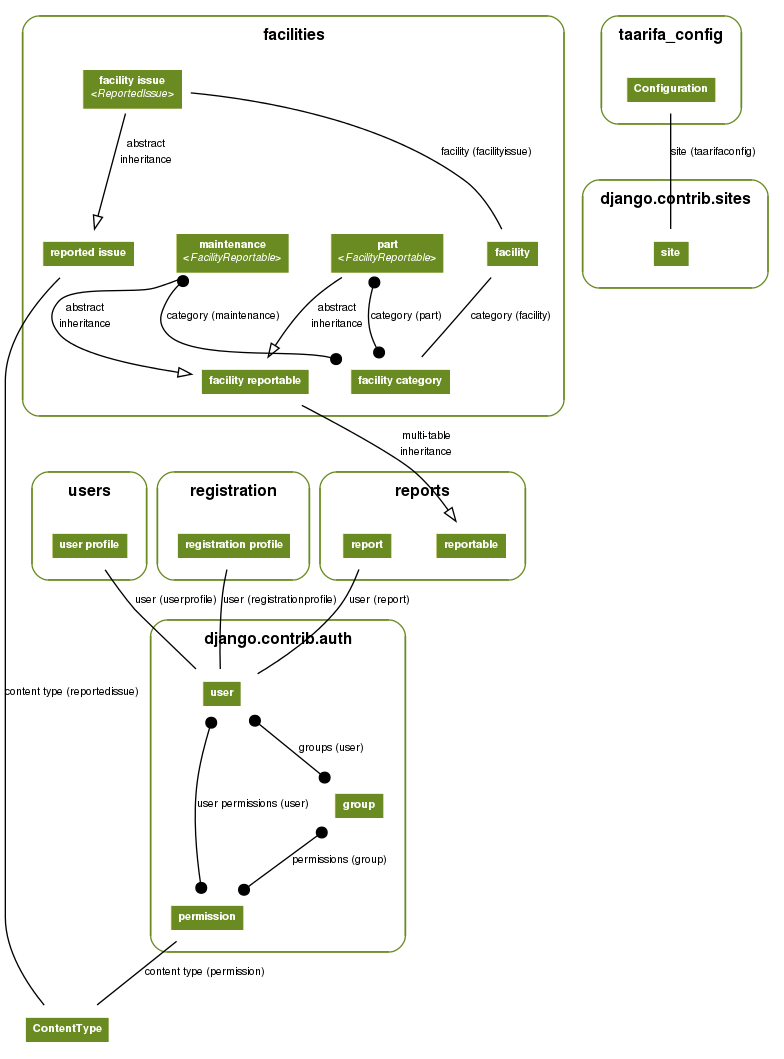
\includegraphics[scale=0.4]{img/overview.png}
\caption{UML Diagram of the overview of the system}
\label{fig:di:uml}
\end{figure}

\FloatBarrier

\subsection{django.contrib.sites}
This is a Django-provided app framework which allows multiple websites to run off the same code. For more information, see \url{https://docs.djangoproject.com/en/dev/ref/contrib/sites/?from=olddocs}.

\subsection{taarifa\_config}
This app was written for an administrator to configure site specific settings. It uses django.contrib.sites to provide different configuration options for different sites using the same database. (Section~\ref{sec:di:admin})

\subsection{facilities}
Facilities management app. Some of its models subclass models provided by reports. (Chapter~\ref{sec:rm})

\subsection{reports}
Reports management app. (Chapter~\ref{sec:rm})

\subsection{registration}
Third-party app called ``django-registration"~\cite{registration} which provides user registration. Parts of it have been overwritten to tailor to Djangorifa. (Section~\ref{sec:di:login})

\subsection{django.contrib.auth}
Django-provided app which provides User, Group and Permission models which are editable through the administration interface. (Section~\ref{sec:di:login}). The ContentType which it points to is an app, django.contrib.contenttypes\footnote{ \url{https://docs.djangoproject.com/en/dev/ref/contrib/contenttypes/}} which is used by Django to keep track of the models in the system.

\subsection{users}
This app was written to provide user profiles so a user can provide additional information about themselves that does not come with django.contrib.auth. (Section~\ref{sec:di:login})

\section{User Registration and Login}
\label{sec:di:login}

Django's default authentication system and django-registration both assume the use of an email address to register, when mobile phones will be the primary method of interaction with the system.

Django.contrib.admin provides:
\begin{itemize}
\item A User model with the required fields: username, password and email address.
\item A Group and Permission model (Section~\ref{sec:di:login:gp})
\end{itemize}

Django-registration provides:
\begin{itemize}
\item Functionality for registering (this is not Django default behaviour)
\item Email address verification
\item Password hashing
\item Password reset
\end{itemize}

It is assumed that users will register with and interact with the system using their mobile phones. Therefore, the registration process had to be changed so as to allow mobile phone number registration.

The users app contains a class called ``MobilePhoneBackend" which is called when a user wants to register. This returns a form ``UserRegistrationForm" when the user views the registration page. The form changes the username field to pass validation only if every character is an integer. The email address field is removed.

When this form is submitted, the email address is saved as the mobile phone number ``@glassberg-powell.com\footnote{My own domain}", for testing purposes. An SMS gateway could be purchased which enables text messages to be sent and received through a website. A few were researched which offered SMS via email. However, they cost money to sign up for, and until the funding is there, the email address will remain as is.

The emails are placed into a task queue by an app called django-mailer~\cite{mailer}. The queue is cleared every 5 minutes by an asynchronous task manager, django-celery~\cite{celery}.

The conceived work-flow is: An SMS will be sent to their phone which they reply to, confirming their phone number.

Django-registration provides an administration interface, but is kept separately from the Django-provided ``User" administration. This is not desired because it separates components which are intrinsically linked. For this reason, the default admin and registration admin interfaces have been disabled, and a custom one written to combine their functionalities.

\subsection{Group and Permission}
\label{sec:di:login:gp}

Groups define groups to which Users can belong. Each Group can have many Permissions which indicate what a User can and cannot do. Every model is automatically created with ``add", ``change" and ``delete" permissions; more can be defined.

Django comes with a super-user and  administrator groups, so ``Citizen" has been defined which provides the permission to make reports. When a user is created, they are automatically added to this group. Permissions to delete or change reports are disabled for transparency reasons. (Appendix~\ref{app:corruption})

\subsection{Profiles}
\label{sec:profiles}

The UML for this app is in Figure~\ref{fig:users}. UserProfile is defined which contains optional details a user may enter about themselves. Future version of Djangorifa might become more of a social network.

\begin{figure}
\centering
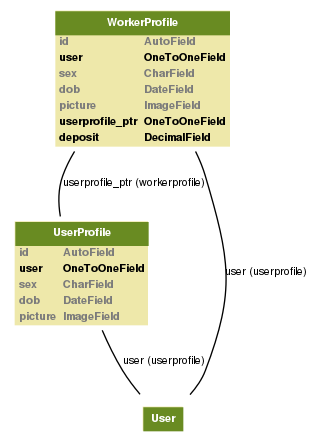
\includegraphics[scale=0.51]{img/users.png}
\caption{Figure to show UML for the users app}
\label{fig:users}
\end{figure}

\section{Administration and Configuration}
\label{sec:di:admin}

\subsection{django.contrib.admin}
An app registers with the admin section through its ``admin.py" file. Classes are defined which allow complete control over the behaviour of models in the admin site. \\

The admin site automatically creates a view to list all instances of a registered model. If one of these instances is clicked on, the user sees a change form for that instance. \\

A third-party app called ``django-grappelli" has been installed which has many additional features, one of which is a search bar on all foreign key relations. For example, ExampleModel1 has a foreign key field to ExampleModel2. There are 10,000 instances of ExampleModel2 in the database. When an administrator wants to add a new ExampleModel1 with the foreign key to an existing ExampleModel2 instance, Django's default behaviour is a drop-down select list. Grappelli replaces that with a search button that can search all columns of a model. \\

Grappelli also changes the theme of the admin site.

\subsection{taarifa\_config}
\begin{figure}
\centering
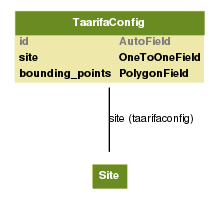
\includegraphics[scale=0.51]{img/config.png}
\caption{UML of taarifa\_config}
\label{fig:taarifa_config}
\end{figure}
An administrator must configure the system on first use. The system will show a message informing them that the site is not configured until they configure. An administrator must choose a site to configure Taarifa for. On the configuration page, an administrator is presented with a map onto which they can draw a polygon to outline the area in which reports can be made. \\

This is used when presenting facilities to a user to report. Only facilities defined in this area will be shown. This is for the case when there are multiple sites running from the same database. \\

The map is provided by a third-party plugin called ``django-olwidget"~\cite{olwidget}. \\

An app can implement a model which has a field with a one-to-one relationship with TaarifaConfig (Figure~\ref{fig:taarifa_config}). This model will automatically be displayed on the configuration page, which enables app-specific settings. This is used by auctions.

\section{Mobile phone version}
\label{sec:di:mobile}

Django has a middleware framework, which provides an \gls{API} for apps to alter request objects before they are passed to views. django-mobile~\cite{mobile} uses this to add a ``flavour" to each request object, which can either be ``mobile" or ``full". Throughout Taarifa, if there are separate views for mobile phones, this feature is used.